\begin{activite}[Additions et soustractions]

\begin{partie}[Première partie : Dénominateurs n'ayant pas de diviseur commun autre que 1]

\begin{center}
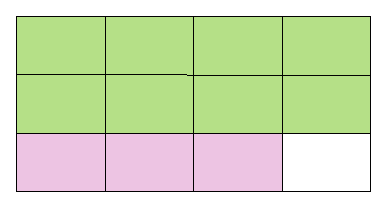
\includegraphics[width=.3\linewidth]{actiADF1}
\end{center}

\begin{enumerate}
\item Complète les phrases suivantes :
    \begin{itemize}
        \item L'aire de la région verte représente $\dfrac{2}{...}$ de l'aire totale ;
        \item L'aire de la région rose représente $\dfrac{1}{...}$ de l'aire totale.
    \end{itemize}
\item \label{ASFacti1} Quel calcul permet d'obtenir l'aire que représente la région coloriée par rapport à l'aire totale ?
\item En t'aidant du dessin, complète l'égalité : $\dfrac{2}{3}+\dfrac{1}{4}=\dfrac{...}{...}$.
\item \label{ASFacti2} Comment retrouver ce résultat par le calcul ?
\end{enumerate}
\end{partie}

\begin{partie}[Deuxième partie : Dénominateurs ayant plusieurs diviseurs communs]
\begin{enumerate}
\item Sur le même rectangle, on veut colorier, en bleu, $\dfrac{1}{8}$ de l'aire et, en orange, $\dfrac{5}{6}$ de l'aire. Quelles dimensions minimales, en nombre entier de centimètres, peux-tu donner à ce rectangle pour que ce partage soit facile à effectuer ? Fais une figure.
\item Reprends les questions \ref{ASFacti1} à \ref{ASFacti2} de la première partie.
\end{enumerate}
\end{partie}

\begin{partie}[Troisième partie : Bilan]
\begin{enumerate}
\item Énonce une règle qui permet d'additionner ou de soustraire des fractions de dénominateurs différents.
\item Applique cette règle pour effectuer les calculs suivants : $\dfrac{1}{5}+\dfrac{7}{2}$ et $\dfrac{7}{10}-\dfrac{11}{15}$.
\end{enumerate}
\end{partie}
\end{activite}





\begin{activite}[Aire d'une portion de disque]

\begin{partie}
\begin{enumerate}
\item Calculer l'aire et le périmètre d'un disque de rayon 9\,cm. On utilisera $\pi \approx 3,14$.
\item Sachant que le rayon mesure 9\,cm, calculer la longueur de l'arc de cercle $AB$ et l'aire du secteur de disque délimité par les rayons $[OA]$ et $[OB]$, et l'arc $AB$, dans chacun des cas suivants :

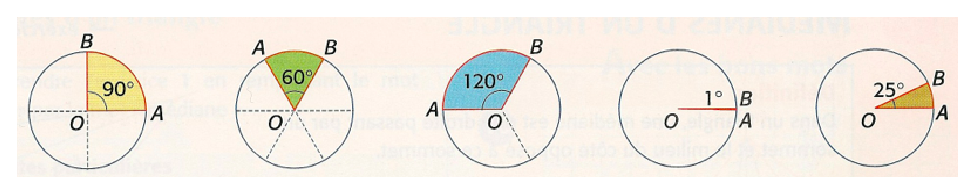
\includegraphics[width=\linewidth]{actiADF2}

\end{enumerate}
\end{partie}

\begin{partie}
L'aire d'un secteur de disque $AOB$ est-elle proportionnelle à la mesure de son angle $\widehat{AOB}$ ? Et la longueur de l'arc $AB$ ?
\end{partie}


\end{activite}
